%%%%%%%%%%%%%%%%%%%%%%%%%%%%%%%%%%%%%%%%%%%%%%%%%%%%%%%%%%%%%%%%%%%%%%%%%%%%%%%
% Chapter 3: Procedimiento experimental 
%%%%%%%%%%%%%%%%%%%%%%%%%%%%%%%%%%%%%%%%%%%%%%%%%%%%%%%%%%%%%%%%%%%%%%%%%%%%%%%

Este cap�tulo ha de contar con seccciones para la descripci�n de los experimentos 
y del material.
%
Tambi�n debe haber una secci�n para los resultados obtenidos y una �ltima de 
an�lisis de los resultados.

%++++++++++++++++++++++++++++++++++++++++++++++++++++++++++++++++++++++++++++++
\section{Descripci�n de los experimentos}
\label{3:sec:1}

bla, bla, etc. 

%++++++++++++++++++++++++++++++++++++++++++++++++++++++++++++++++++++++++++++++
\section{Descripci�n del material}
\label{3:sec:2}

bla, bla, etc. 


%++++++++++++++++++++++++++++++++++++++++++++++++++++++++++++++++++++++++++++++
\section{Resultados obtenidos}
\label{3:sec:3}

bla, bla, etc. 


%------------------------------------------------------------------------------
\begin{figure}[!th]
\begin{center}
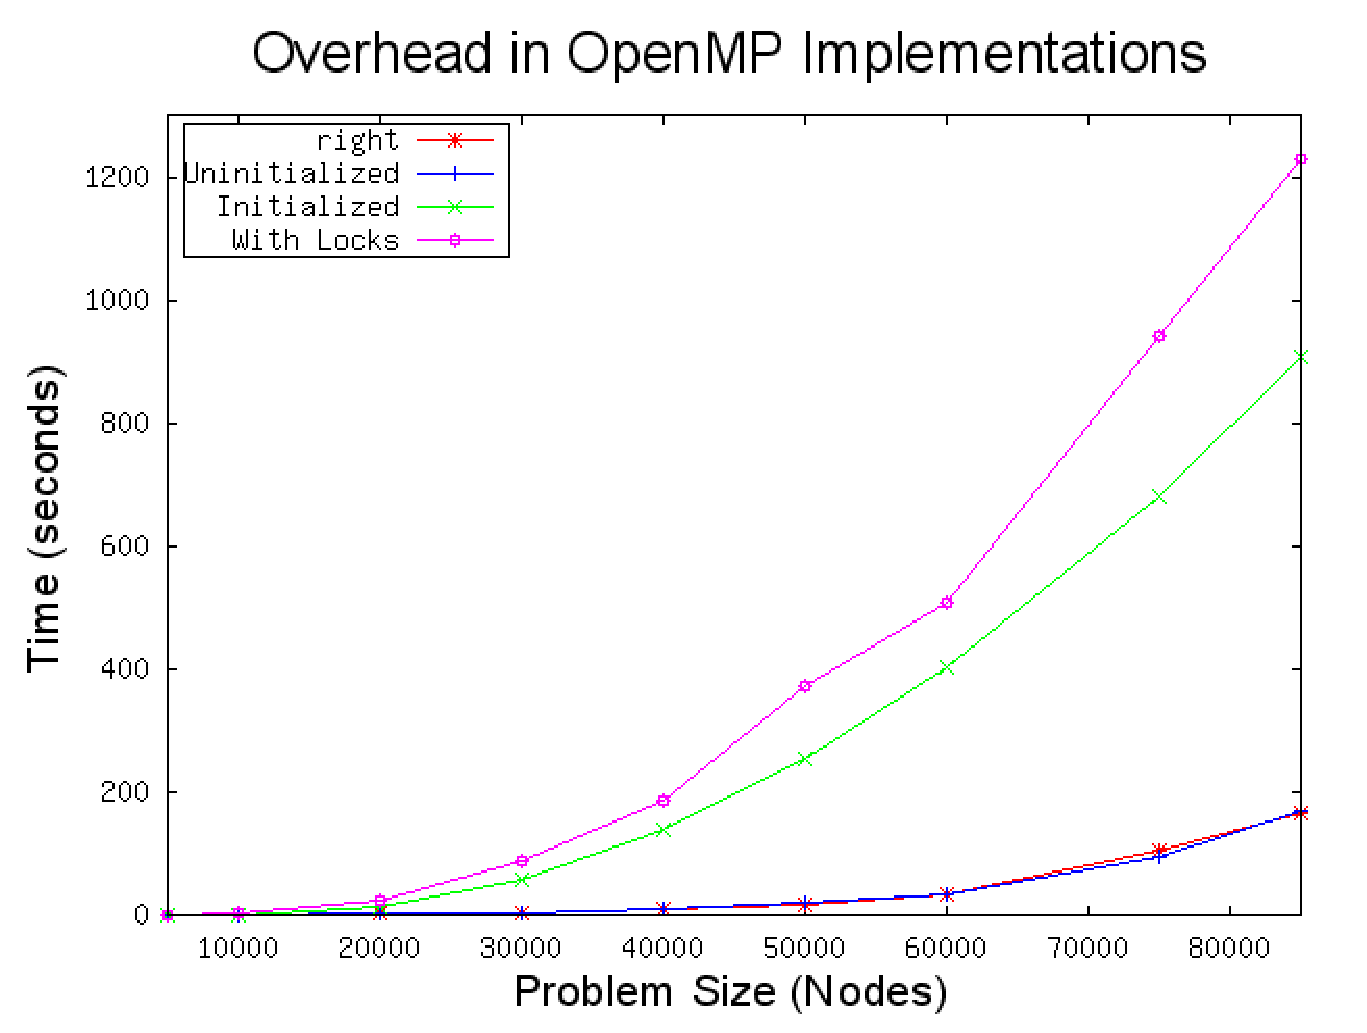
\includegraphics[width=0.75\textwidth]{images/figura1.eps}
\caption{Ejemplo de figura}
\label{fig:1}
\end{center}
\end{figure}
%------------------------------------------------------------------------------


%------------------------------------------------------------------------------
%--------------------------------------------------------------------------
\begin{table}[!ht]
\begin{center}
\begin{tabular}{|c|c|} \hline 
\textbf{Tiempo  } & \textbf{Velocidad} \\ 
\textbf{($\pm$ 0.001 s)} & \textbf{($\pm$ 0.1 m/s)} \\ \hline \hline
1.234 &
67.8
\\
\hline

2.345 &
78.9
\\
\hline

3.456 &
89.1
\\
\hline

4.567 &
91.2
\\
\hline

\end{tabular}
\end{center}
\caption{Resultados experimentales de tiempo (s) y velocidad (m/s)}
\label{tab:1}
\end{table}


%------------------------------------------------------------------------------

%++++++++++++++++++++++++++++++++++++++++++++++++++++++++++++++++++++++++++++++
\section{An�lisis de los resultados}
\label{3:sec:4}

bla, bla, etc. 

